\chapter{Experimentations with SLM}
\label{chp:SLM}
\section{Initial Experiments to image mask}
The experimental setup consists of a coherent laser beam, two mirrors, a spatial filter, a collimator lens, LC2012 SLM and finally an OV2640 CMOS sensor. The experimental setup is shown in Figure \ref{fig:experiment_slm}. The collimator lens and the spatial filter make the beam parallel and remove unwanted random noise in the laser beam.

\begin{figure}[htbp]
\centering
\includegraphics[width = 0.75\linewidth]{pics/slm_experiment}
\caption{Experimental Setup to image mask}
\label{fig:experiment_slm}
\end{figure}

I started off the experiment with the setup shown in Figure \ref{fig:experiment_slm}. However, when trying to take an image of the mask with the CMOS sensor, I faced multiple challenges along the way. The first challenge came in the form of the memory limitations of the camera module. The OV2640 camera module has only 384KB of memory which can store compressed JPEG images when imaging with the lens. The memory limitation of the camera does not come into effect when imaging with the lens as JPEG encoding is naturally designed for reducing the size of real-life artifacts and object scenes with a very high compression ratio. However, when using the same camera module, for lensless imaging, the size of the image easily exceeds the size of the FIFO buffer and the host software provided by the vendor is unable to read out the images. In order to overcome this challenge, I thought of increasing the extent of compression(with a trade-off of loss in quality) to image the mask. This can be done by changing the \texttt{QSC} register(quantization scale factor) \cite{OV2640DS} of the CMOS sensor. The default value of the quantization scale factor is \texttt{0C}(hex value). This value was increased to \texttt{2F} by setting the registers using I2C as mentioned for the previous acceptance cone experiments. The size of the image was successfully reduced and the host software was able to read out images. After this, the sensor was placed in front of the SLM and the experiments were continued. I started experimenting with the default masks provided by the SLM vendor before continuing onto the custom mask designed using simulations. The mask that was used is a binary axicon mask and binary mask which divides the SLM into two different halves.The figure of the mask is shown in Figure \ref{fig:InitMask}. 

After overcoming this challenge I faced the second challenge wherein, the binary axicon mask was not visible and the central part of the sensor had saturated(whited out). This can be seen in Figure \ref{fig:InitMaskCMOS}. It can be seen from Figure \ref{fig:InitMaskCMOS} that the binary axicon mask is not at all visible due to the saturation of the CMOS sensor in the central region. The horizontal mask is imaged as a vertical mask by the CMOS sensor as the SLM is oriented vertically against the CMOS sensor. Even in the horizontal mask, the central portion has saturated. 

\begin{figure}[h]
    \centering
    \begin{subfigure}{0.5\textwidth}
    \centering
        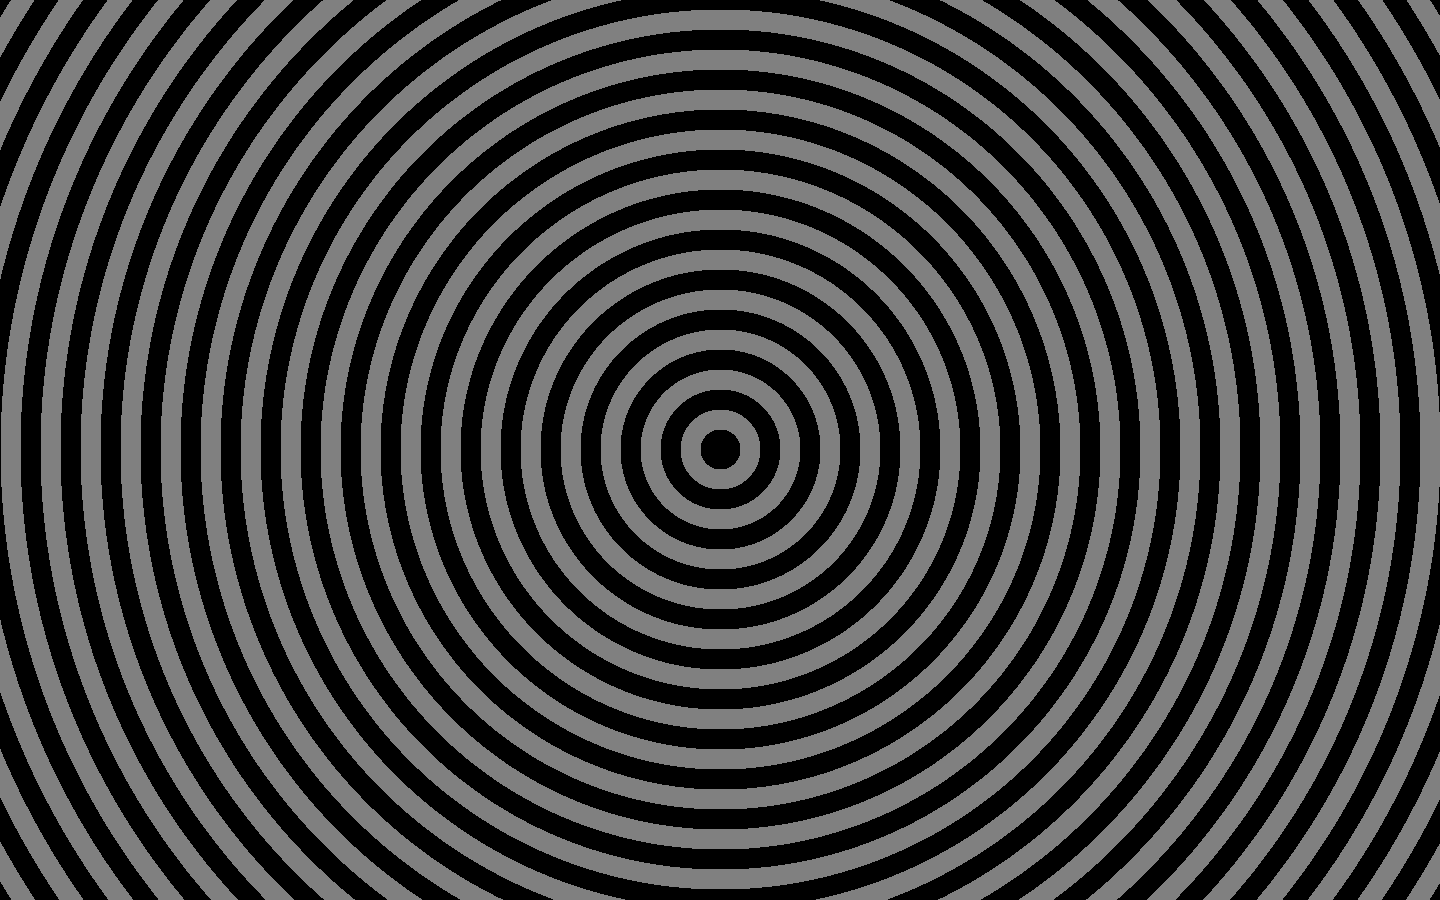
\includegraphics[width=0.5\linewidth]{pics/slm/binaryaxicon.png}
        \caption{Binary Axicon Mask}
        \label{fig:axiconmask}
    \end{subfigure}%
    \begin{subfigure}{0.5\textwidth}
    \centering
        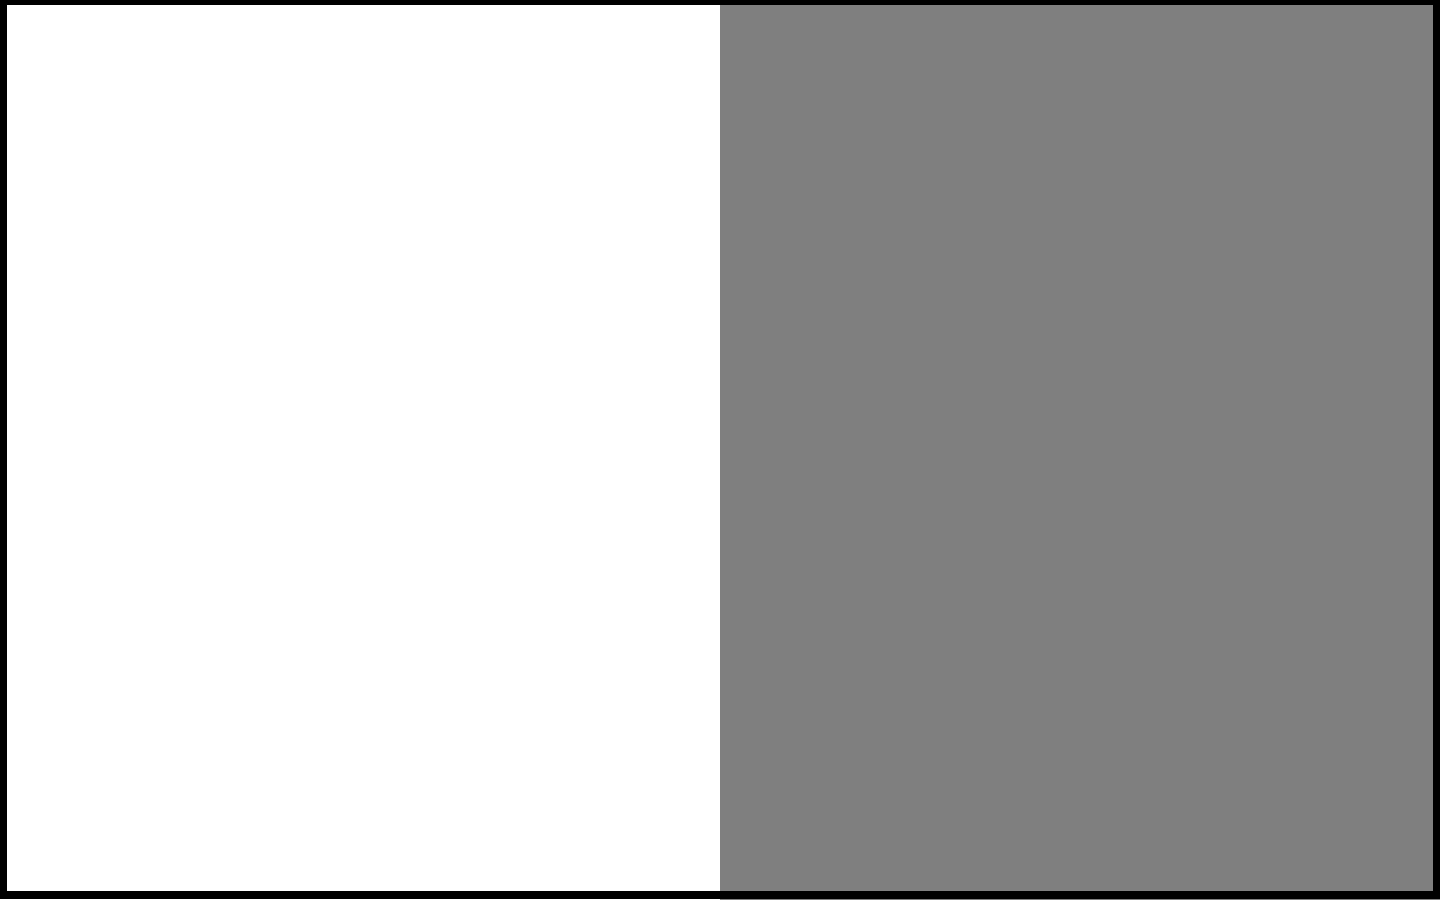
\includegraphics[width=0.5\linewidth]{pics/slm/hor-div.png}
        \caption{Horizontal dividable mask}
        \label{fig:hordivmask}
    \end{subfigure}
    \caption{Binary Masks used for Test}
    \label{fig:InitMask}
    \end{figure}
    
    \begin{figure}[h]
    \centering
    \begin{subfigure}{0.5\textwidth}
    \centering
        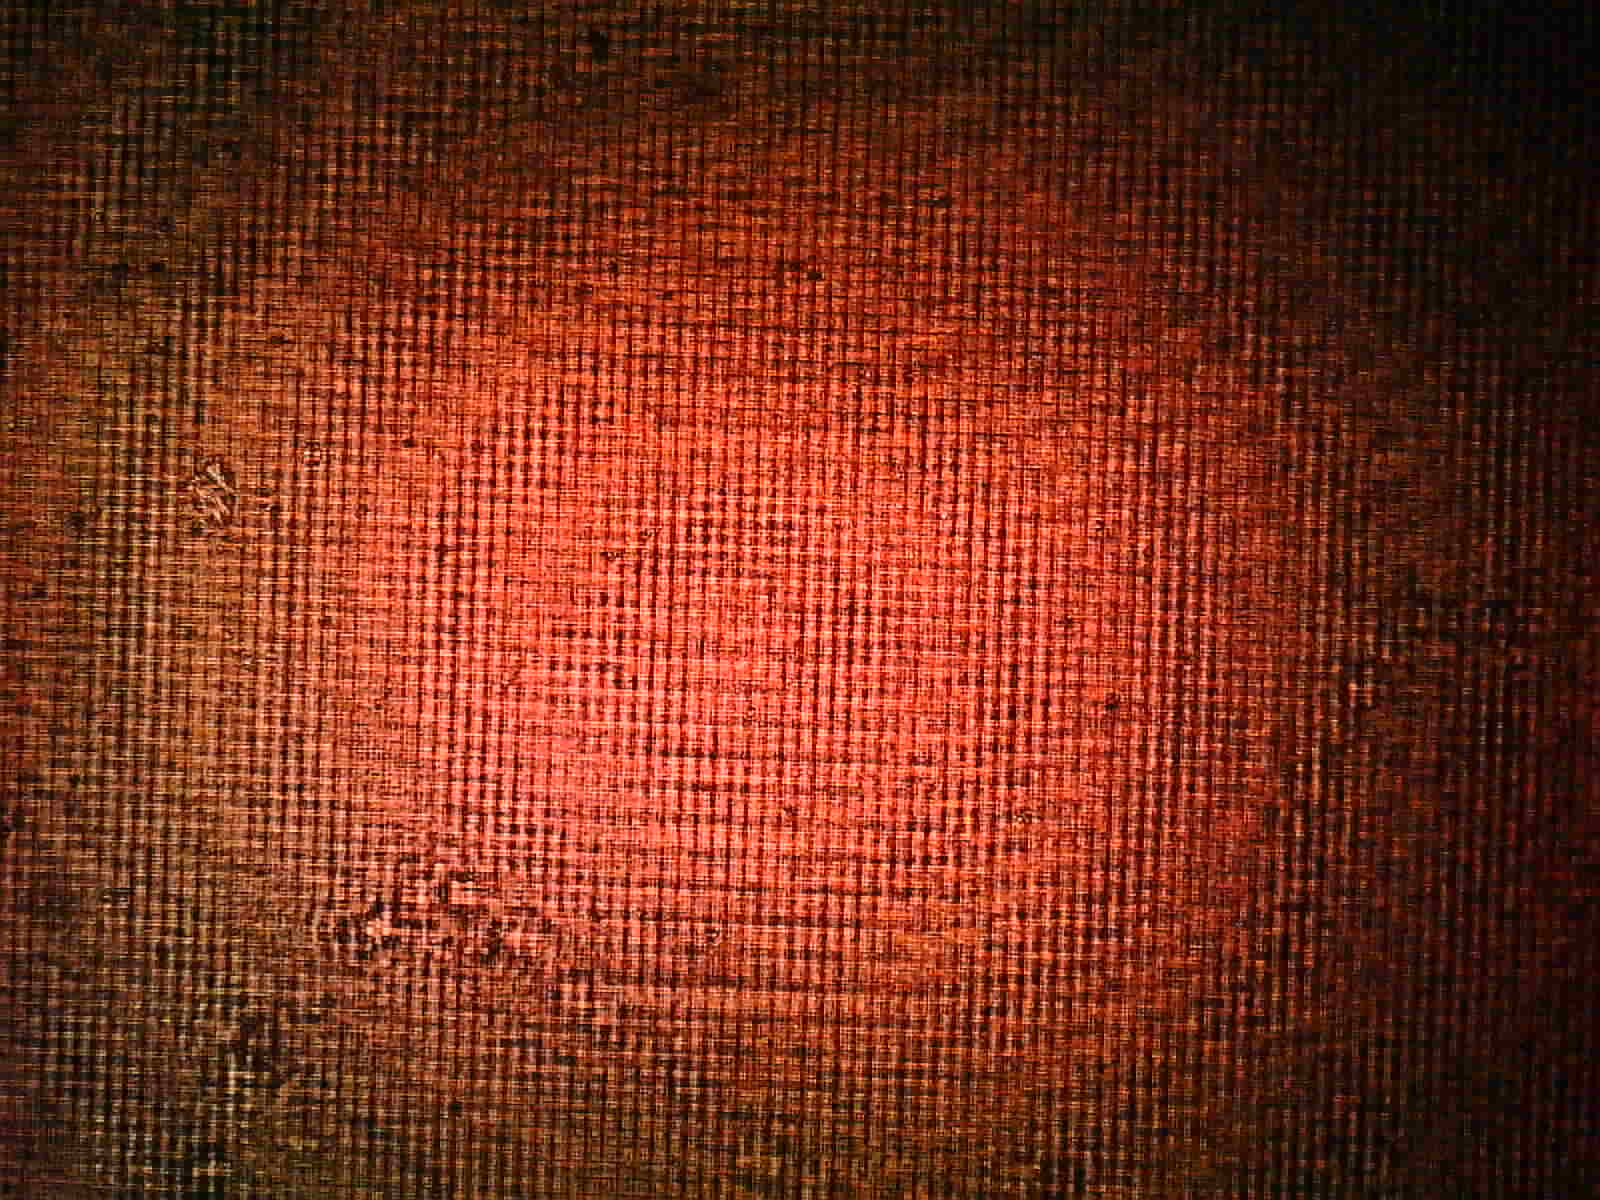
\includegraphics[width=0.5\linewidth]{pics/slm/binaryaxiconcmos.jpg}
        \caption{Binary Axicon Mask imaged by CMOS}
        \label{fig:binaryaxiconcmos}
    \end{subfigure}%
    \begin{subfigure}{0.5\textwidth}
    \centering
        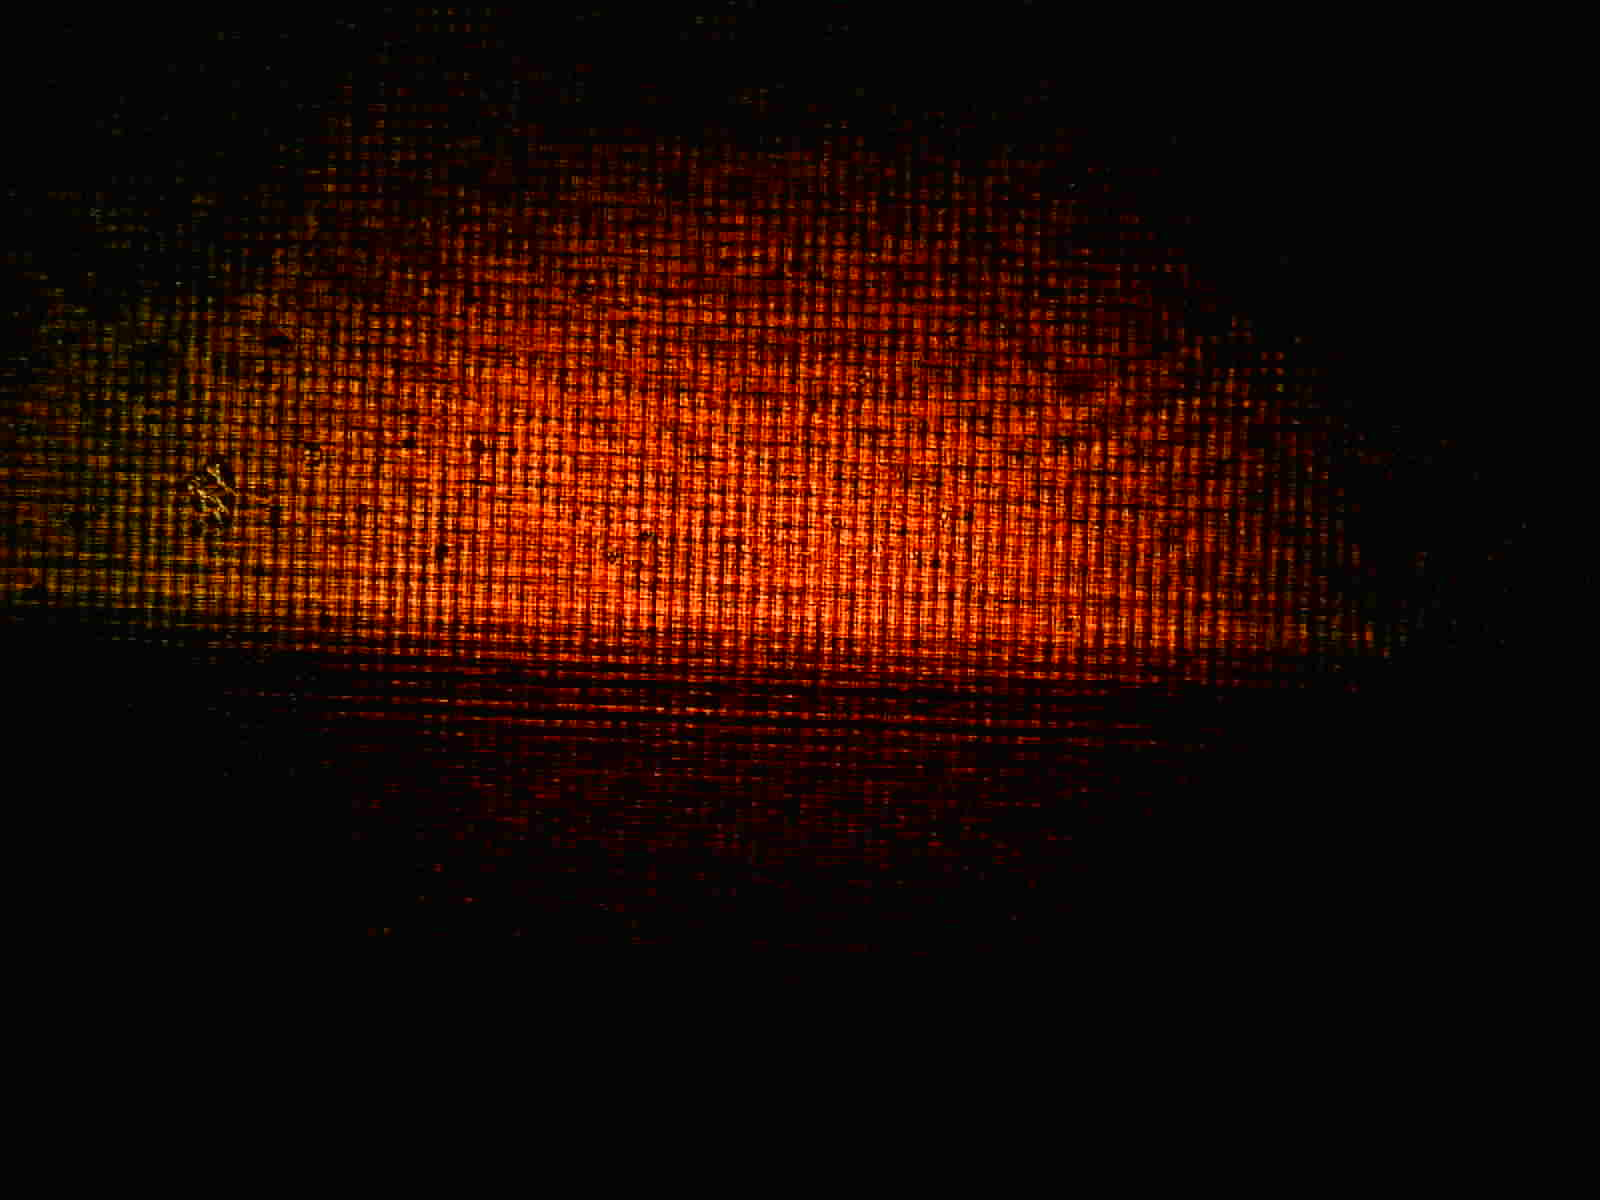
\includegraphics[width=0.5\linewidth]{pics/slm/horizontalcmos.jpg}
        \caption{Horizontal dividable mask imaged by CMOS}
        \label{fig:hordivmask}
    \end{subfigure}
    \caption{Binary Masks used for Test}
    \label{fig:InitMaskCMOS}
    \end{figure}
In order to solve these problems, multiple changes were made to the way the experiment was conducted. To avoid saturation, the exposure time of the CMOS sensor was reduced to the least possible value(70 $\mu$seconds). Since this did not affect the image of the mask formed on the sensor, it was decided to change the brightness and contrast levels of the SLM itself. The transmissive SLM acts as an LCD screen and thus it has its own brightness and contrast levels that affect the amount of light reaching the sensor. So, I decided to study the effect of the brightness and contrast of the image sensor. Also, two n.d filters were added to the setup that cut the intensity of light reaching the sensor by 75 percent. The SLM was placed approximately at a distance of 1 $cm$(10 $mm$) from the image sensor for these experiments. It could not be moved closer than 1 cm because the SLM is covered with polarizers to filter the light reaching the sensor and to prevent any damage to the SLM.

\section{Effect of SLM brightness and contrast on CMOS sensor}
The first set of experiments was conducted to see the effect of brightness and contrast of the SLM on the image formed by the CMOS sensor. For this, I thought of illuminating the CMOS sensor using the laser beam and then study the output image from the CMOS sensor for different gray levels on the CMOS sensor. The highest gray level(255) was chosen and the brightness/contrast levels were varied to see which brightness/contrast levels best represent the amount of light proportional to the grayscale levels of the SLM(i.e. maximum reduction in intensity). A gray level of 255 represents complete blocking of light and a gray level of 0 represents the complete passage of light. The binary mask should be translated to gray levels before we can put it on the SLM. So, we need to study the impact of brightness/contrast on the gray levels. The brightness/contrast levels could be varied from 0 to 64 on the SLM. All the readings were normalized with respect to 255 to see how the intensity drops with respect to grayscale levels. It can be seen from figure \ref{fig:slm_grayscale255} and table \ref{tbl:attenuation255} that there is a certain level of drop in intensity signal irrespective of the brightness levels. It can be seen from Figure \ref{fig:slm_grayscale255} that the maximum brightness and contrast levels best reflect the gray levels of the SLM. 

\begin{figure}[htbp]
\centering
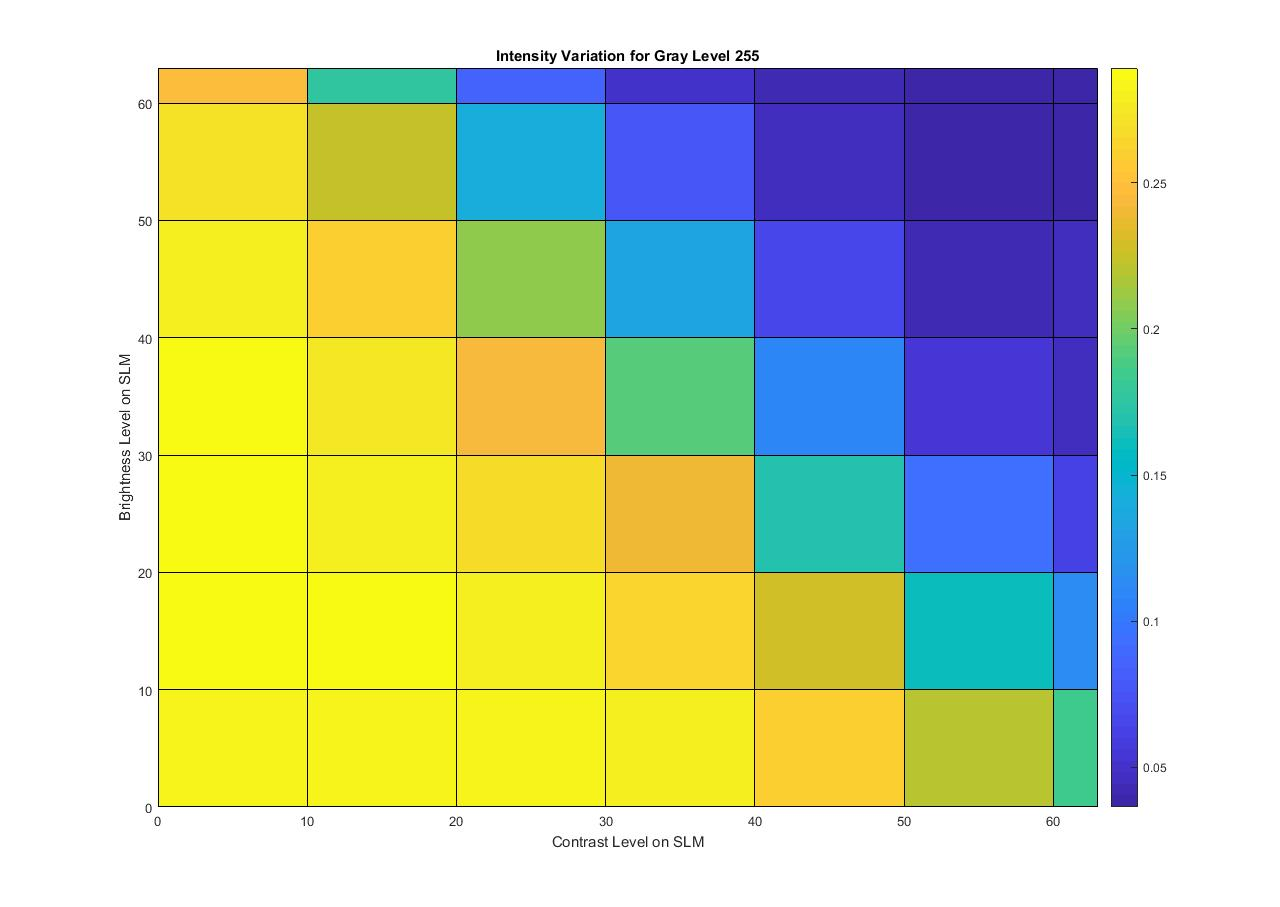
\includegraphics[width = \linewidth]{pics/slm/slmgrayscale255.jpg}
\caption{Effect of brightness and contrast on intensity for grayscale 255}
\label{fig:slm_grayscale255}
\end{figure}


\begin{center}
\begin{table}[!h]
\caption{Attenuation Factors of gray level 255 with respect to gray level 0 for different brightness and contrast levels}
\label{tbl:attenuation255}
\begin{tabular}{|l|*{8}{c|}}\hline
\backslashbox{B}{C}
&\makebox[3em]{0}&\makebox[3em]{10}&\makebox[3em]{20}&\makebox[3em]{30}
&\makebox[3em]{40}&\makebox[3em]{50}&\makebox[3em]{60}&\makebox[3em]{63}\\\hline
\makebox[3em]{0} &0.9834&0.9941&1.3247&1.2975&0.9602&1.0882&    0.81991&0.8124\\\hline
\makebox[3em]{10}&0.9971&1.0161&1.2988&1.2161&0.8096&0.5931&    0.4336&0.3780\\\hline
\makebox[3em]{20}& 1.011&0.9831&1.2162&1.5084&0.5896&0.3460&    0.2686&0.2113\\\hline
\makebox[3em]{30}&0.9966&0.9647&1.1133&0.8718&0.3898&0.2200&0.16253&0.1946\\\hline
\makebox[3em]{40} &0.9841&0.9138&0.9454&0.4592&0.2239&0.1554&0.1627&0.14317\\\hline
\makebox[3em]{50} &0.9350&0.7867&0.6462&0.2665&0.1593&0.1420&0.1296&0.1356\\\hline
\makebox[3em]{60} &0.8626&0.6265&0.3937&0.2237&0.1418&0.1345&0.1327&0.1291\\\hline
\makebox[3em]{63}&0.8188&0.7389&0.3334&0.2104&0.1375&0.1323&0.1385&0.1293\\\hline
\end{tabular}
\end{table}
\end{center}

\section{Effect of gray levels on CMOS sensor}
From the experimental results mentioned in the previous section, it can be seen that the maximum brightness and contrast levels of the SLM provide the maximum attenuation in signals. So, these values were chosen and the grayness levels of the SLM was varied from 0 to 255 and study how the grayscale levels affect the amount of light passing through the SLM. The entire SLM screen is set to this grayscale level so that the entire sensor is modulated with the same intensity of light.
The mean of the entire output image of the CMOS sensor is taken for plotting the signal and it is normalized with respect to the maximum reading and the graph is plotted. This is shown in figure \ref{fig:grayscale_slm_graph}. As it can be seen in the graph, the lowest point corresponds to an intensity reduction of approximately 88 percent. One important observation is that it is not possible to create a completely binary mask which blocks light as the maximum intensity reduction is only 88 percent. This will have an effect on the image reconstruction as it is assumed that the mask is completely binary. 

\begin{figure}[!htbp]
\centering
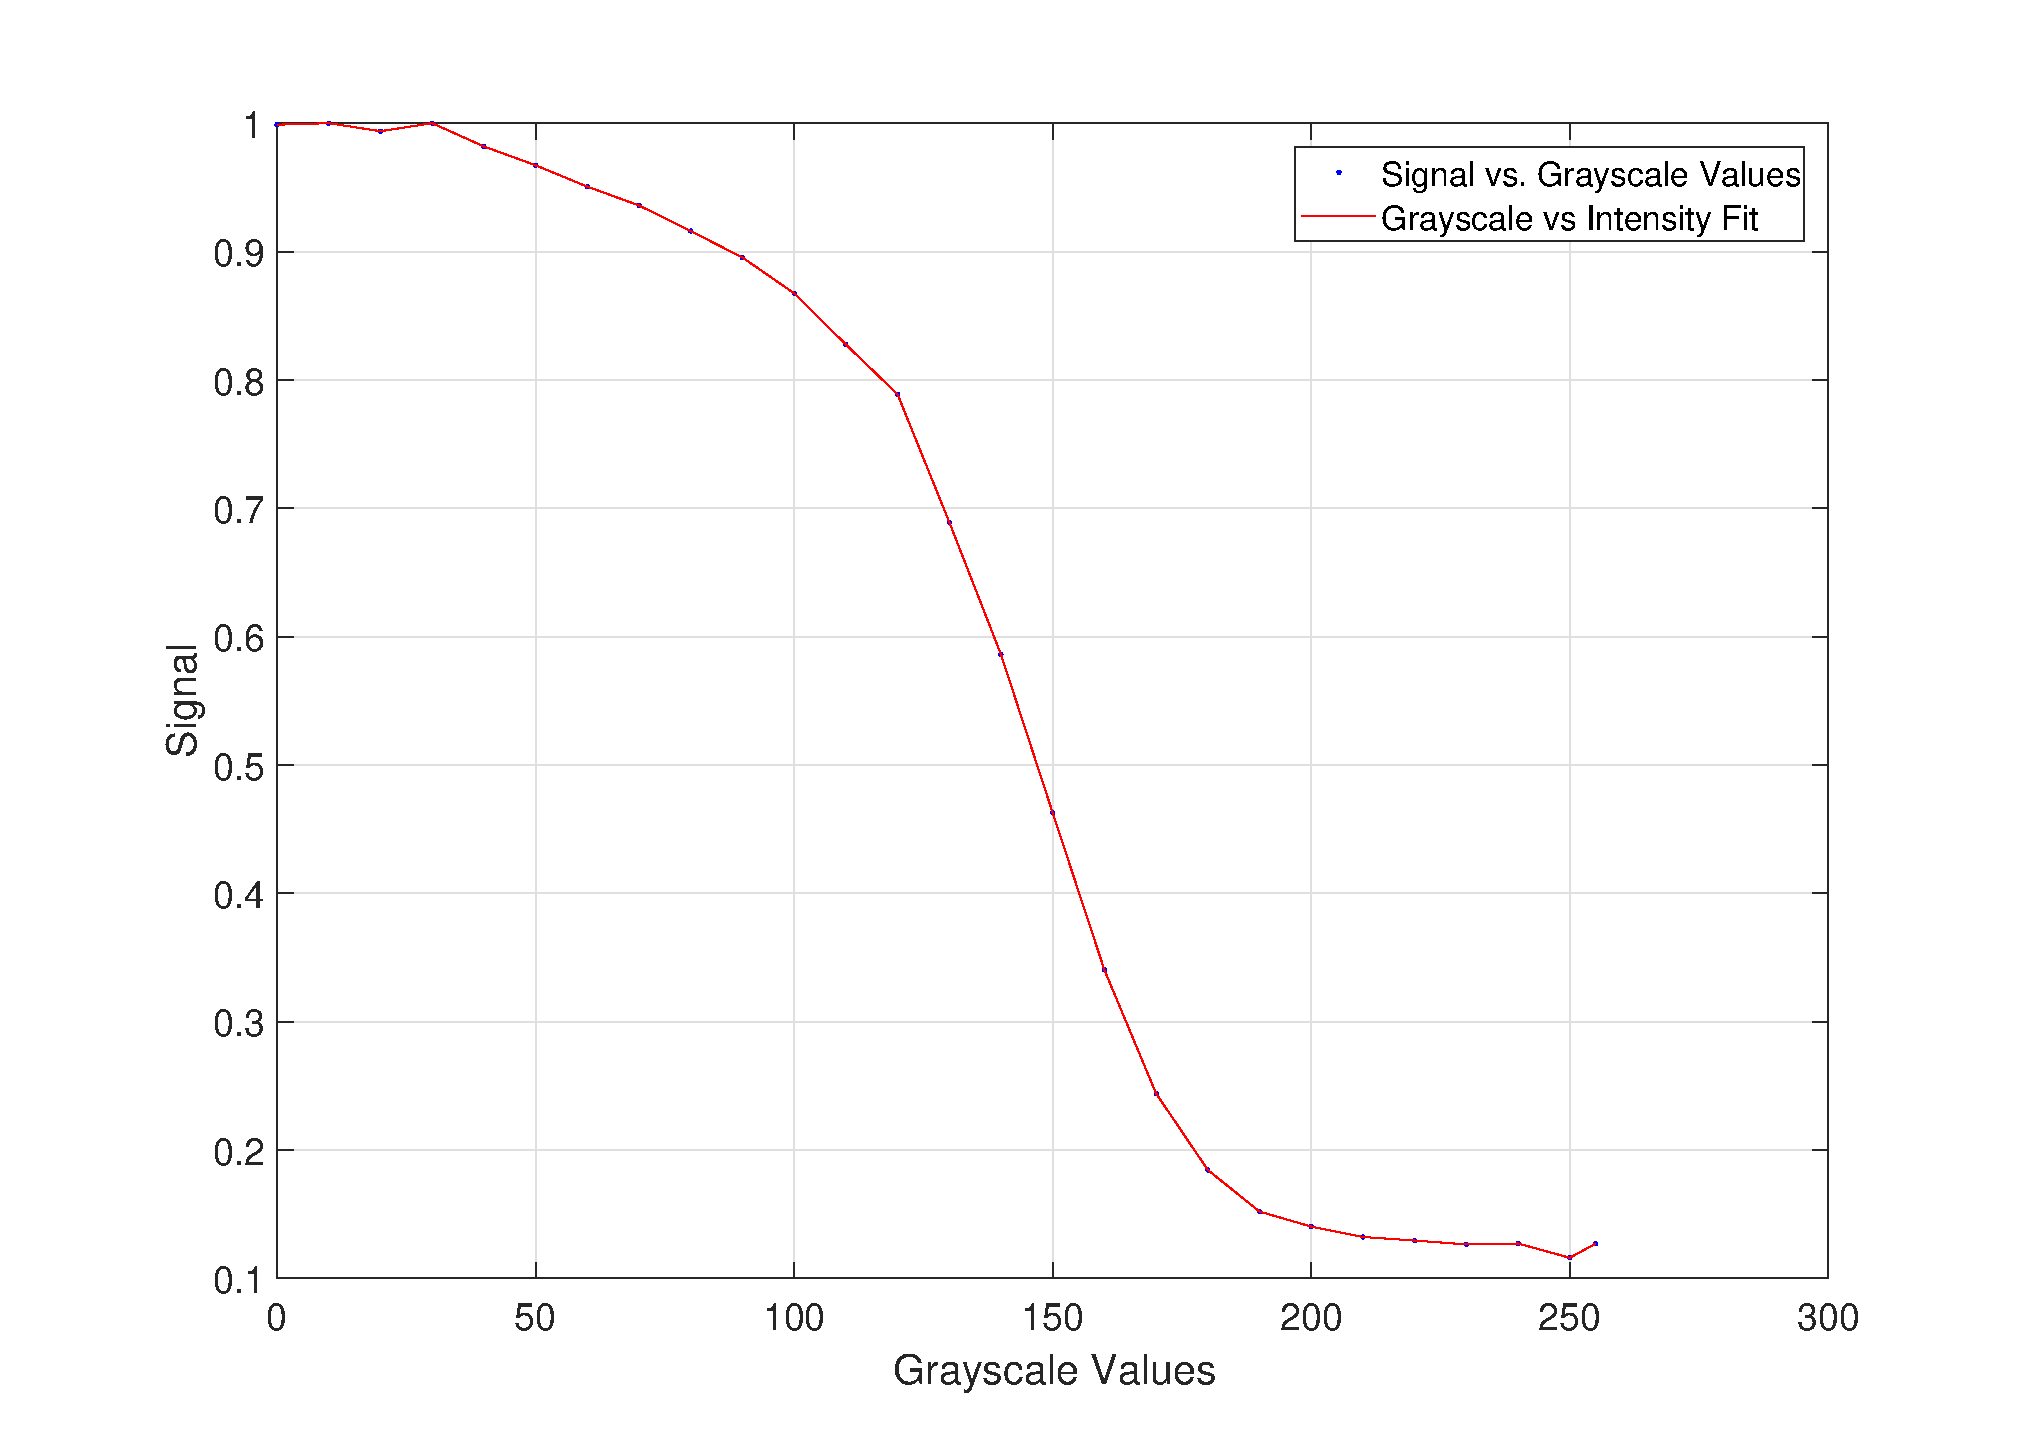
\includegraphics[width = \linewidth]{pics/slm/grayscale_slm_graph}
\caption{Grayscale vs intensity of light received by the CMOS sensor.}
\label{fig:grayscale_slm_graph}
\end{figure}

\section{Imaging of Separable Mask using CMOS sensor}
In the previous section, we discussed how the SLM brightness and contrast affect the mask visibility on the CMOS sensor. In this section, we keep the mask brightness and contrast at maximum possible setting and image the mask. A separable doubly Toeplitz mask is generated for the resolution of the SLM. The generated mask is converted to gray level 255 for regions that block light and gray level 0 for regions that allow light.The gray level mask is then programmed onto the SLM. As mentioned in the previous sections, a doubly Toeplitz mask is one in which the row and column of the matrix can be expressed in the form:

$$
M = A_{1024\times 1}{(B_{768 \times 1})}^T
$$

Like in the simulations, a linearly spaced random vector is generated for a specific length(\texttt{Nxm0}) and interpolated to the SLM screen length(1024 $\times$ 768). Two vectors are generated(keeping \texttt{Nxm0} and \texttt{Nym0} constant) and the outer product of the vectors is taken to produce a mask that is same as the resolution of the SLM.
We need to perform singular value decomposition on the output image from the CMOS sensor in order to make sure that the mask preserves the property of separability. Since the SLM is larger than the CMOS sensor, the sensor only images a particular portion of the mask and not the complete mask itself. The mask can be decomposed into a singular matrix value no matter which part of the mask is imaged by the sensor. This was also verified in the MATLAB simulations by cutting out different portions of the mask and testing for separability. The doubly Toeplitz mask generated and used for the experiments is shown in figure \ref{fig:doubly_toepl_custom}. The region marked in red will also exhibit only one singular value on performing SVD.
\begin{figure}[h]
\centering
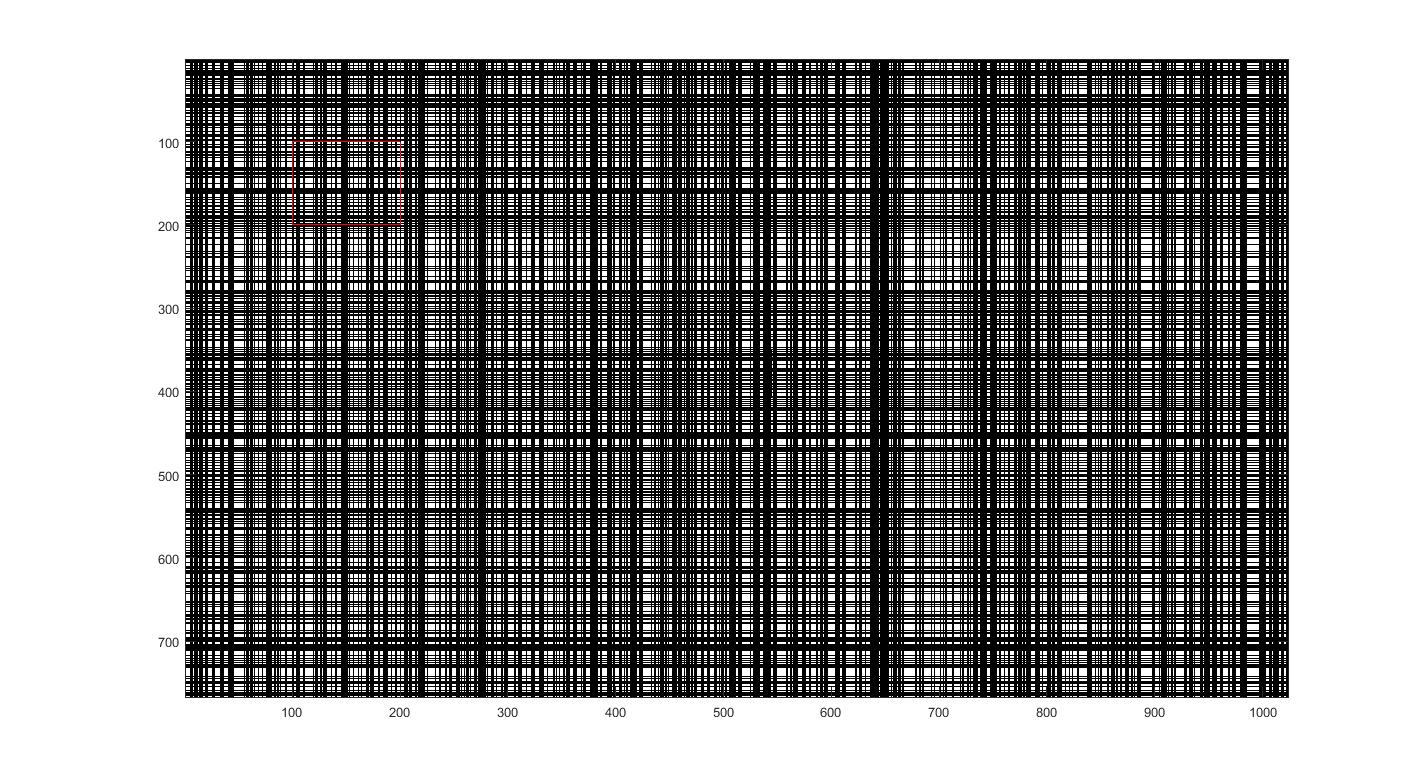
\includegraphics[width = 0.75\textwidth]{pics/slm/mask_sub_prop}
\caption{Doubly Toeplitz mask}
\label{fig:doubly_toepl_custom}
\end{figure}
SVD forms the basis of the mask imaging experiment. We image the mask using OV2640 and see whether the mask still exhibits the same property when imaged by the CMOS sensor. The image of the doubly Toeplitz mask imaged by OV2640 is shown in figure \ref{fig:dt_ov2640}.
\begin{figure}[h]
\centering
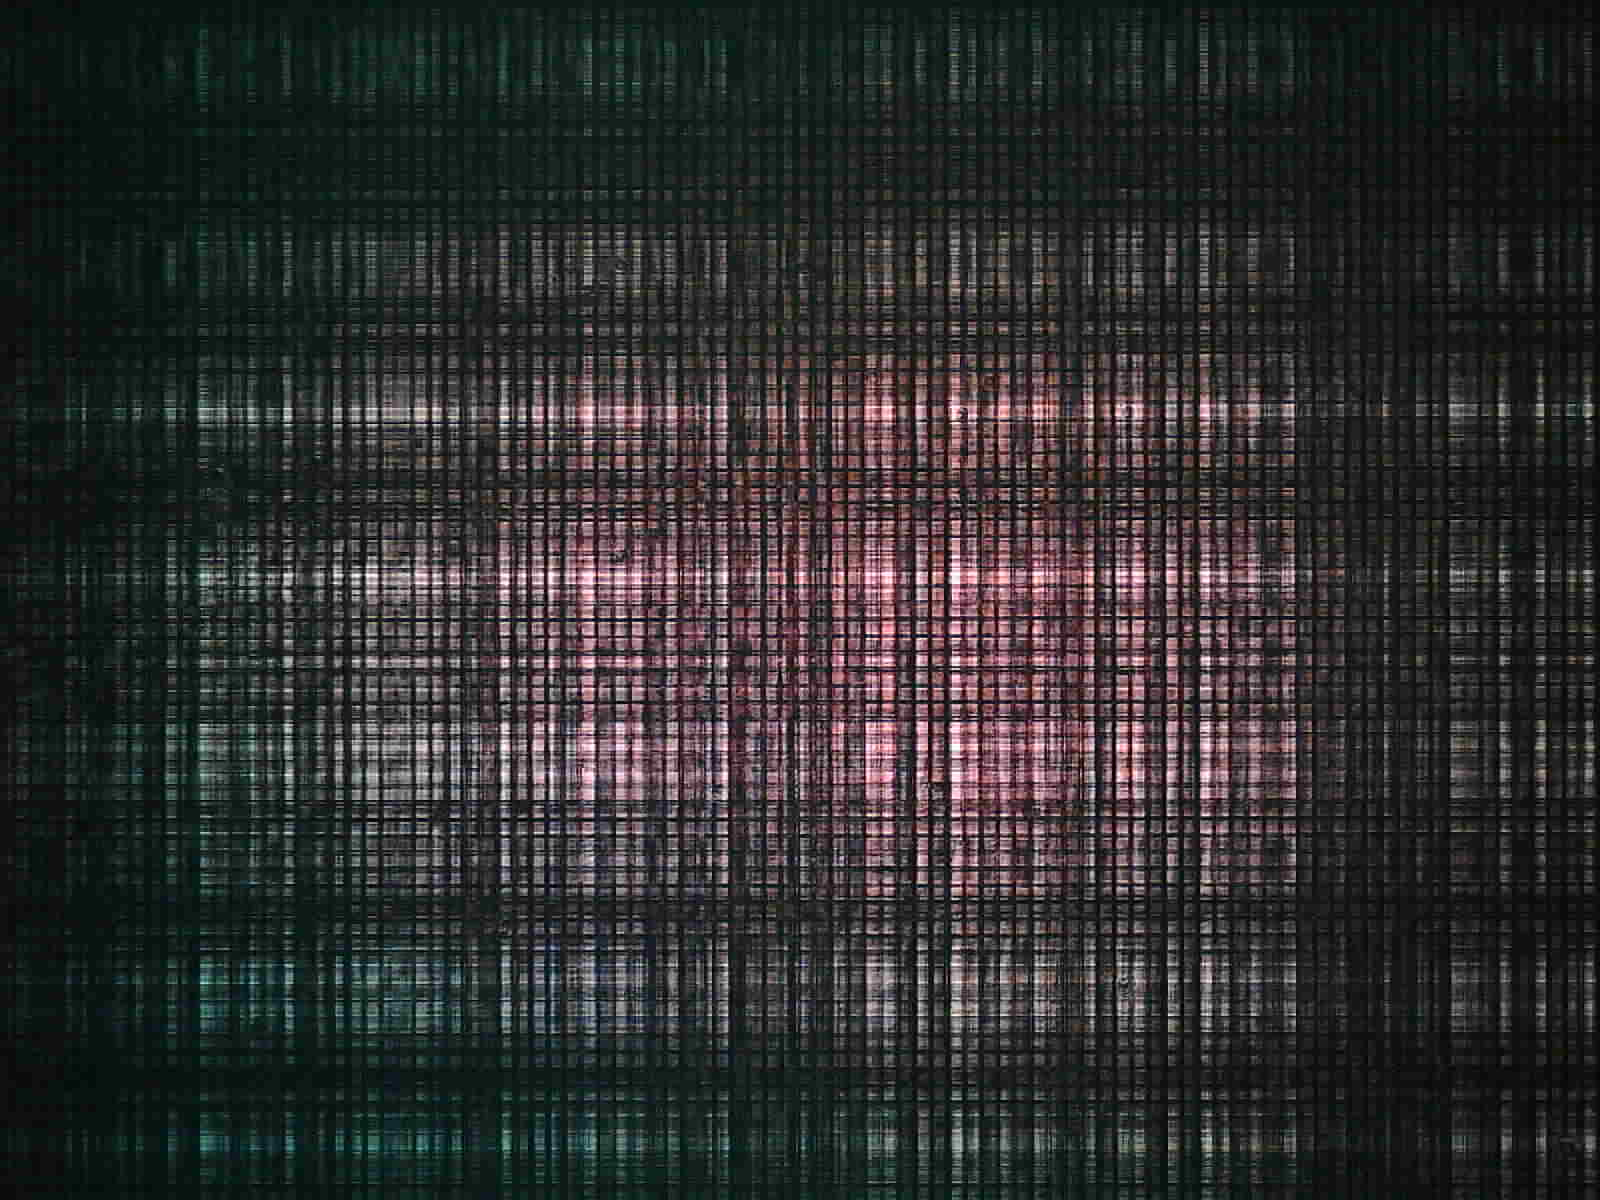
\includegraphics[scale=0.20]{pics/slm/ov2640dtmask.jpg}
\caption{Doubly Toeplitz mask imaged by OV2640 after modification of Q-Table}
\label{fig:dt_ov2640}
\end{figure}
As can be seen from the figure \ref{fig:dt_ov2640}, the OV2640 produces a very poor image of the mask. This can be attributed to the poor quality of compression. The quantization factor increased during the previous experiments(see the first section in this chapter) in order to reduce the size of the image has reduced the quality of the output image. The change in the default quantization matrix and the modified quantization matrix that has been used for compression is shown below. The default quantization matrix has been modified so that the size of the image is within 384 KB. Without modifying the quantization scale factor, it would not be possible to obtain an image using a mask-sensor setup using OV2640. From the modified Q-Table, we can see that the higher frequency components will be eliminated and the lower frequency components will be retained. The Q-tables were obtained using the \texttt{djpeg} program\cite{djpeg} on the output image sensors running on Linux. 
\[
Q-Default = 
\begin{bmatrix}
          12  &  8 &   8  & 12 &  18 &  30 &  38&   46 \\
           9   & 9  & 11  & 14  & 20  & 44   &45  & 41 \\
          11  & 10 &  12  & 18 &  30 &  43 &  52 &  42 \\
          11  & 13  & 17   &22  & 38  & 65  & 60  & 47 \\
          14  & 17  & 28  & 42  & 51 &  82 &  77 &  58 \\
          18  & 26  & 41  & 48 &  61  & 78 &  85  & 69 \\
          37  & 48 &  59 &  65 &  77 &  91 &  90 &  76 \\
          54  & 69  & 71  & 74  & 84  & 75  & 77  & 74 \\
\end{bmatrix}
\]
\[
Q-Modified = 
\begin{bmatrix}
        47 &  32 &  29 &  47 &  71 & 118 & 150 & 179 \\
          35 &  35 &  41 &  56 &  76 & 170 & 176 & 162\\
          41 &  38 &  47  & 71 & 118 & 167 & 203 & 165\\
          41 &  50 &  65  & 85 & 150 & 255 & 235 & 182\\
          53 &  65 & 109 & 165 & 200 & 255 & 255 & 226\\
          71 & 103 & 162 & 188 & 238 & 255 & 255 & 255\\
         144 & 188 & 229 & 255 & 255 & 255 & 255 & 255\\
         212 & 255 & 255 & 255 & 255 & 255 & 255 & 255\\
\end{bmatrix}
\]

Based on the mask image and the quantization tables obtained, we can be sure that it would be impossible to obtain proper reconstructions using OV2640. So, it was decided to try whether other CMOS sensors would produce better quality pictures that would enable proper reconstruction. Based on the trade-off factors discussed previously, an OV5642 sensor was also bought in the case of any failure. Since OV2640 and OV5642 follow the same architecture and use the same open-source libraries, it was easy to port the embedded software from OV2640 and OV5642. Also, APIs are provided to control the exposure level of OV5642 in 10 possible steps. The exposure was set to minimum possible level as higher levels cause saturation of sensor data. The compression quality was set to High using APIs provided by Arducam. It was then decided to check the image quality on OV5642. The OV5642 has an advantage that it has a bigger active sensor array($2592 \times 1944$) and comes with a larger FIFO buffer(8MB). The CMOS sensor needs to be perfectly aligned and the perfect alignment would be given by the maximum singular value ratio. In order to position these sensors on the stage, a script was written that would calculate the singular values in real time. The tilt of the sensor was adjusted such that the ratio of the first component to the second component is maximum. 
\begin{figure}[h]
\centering
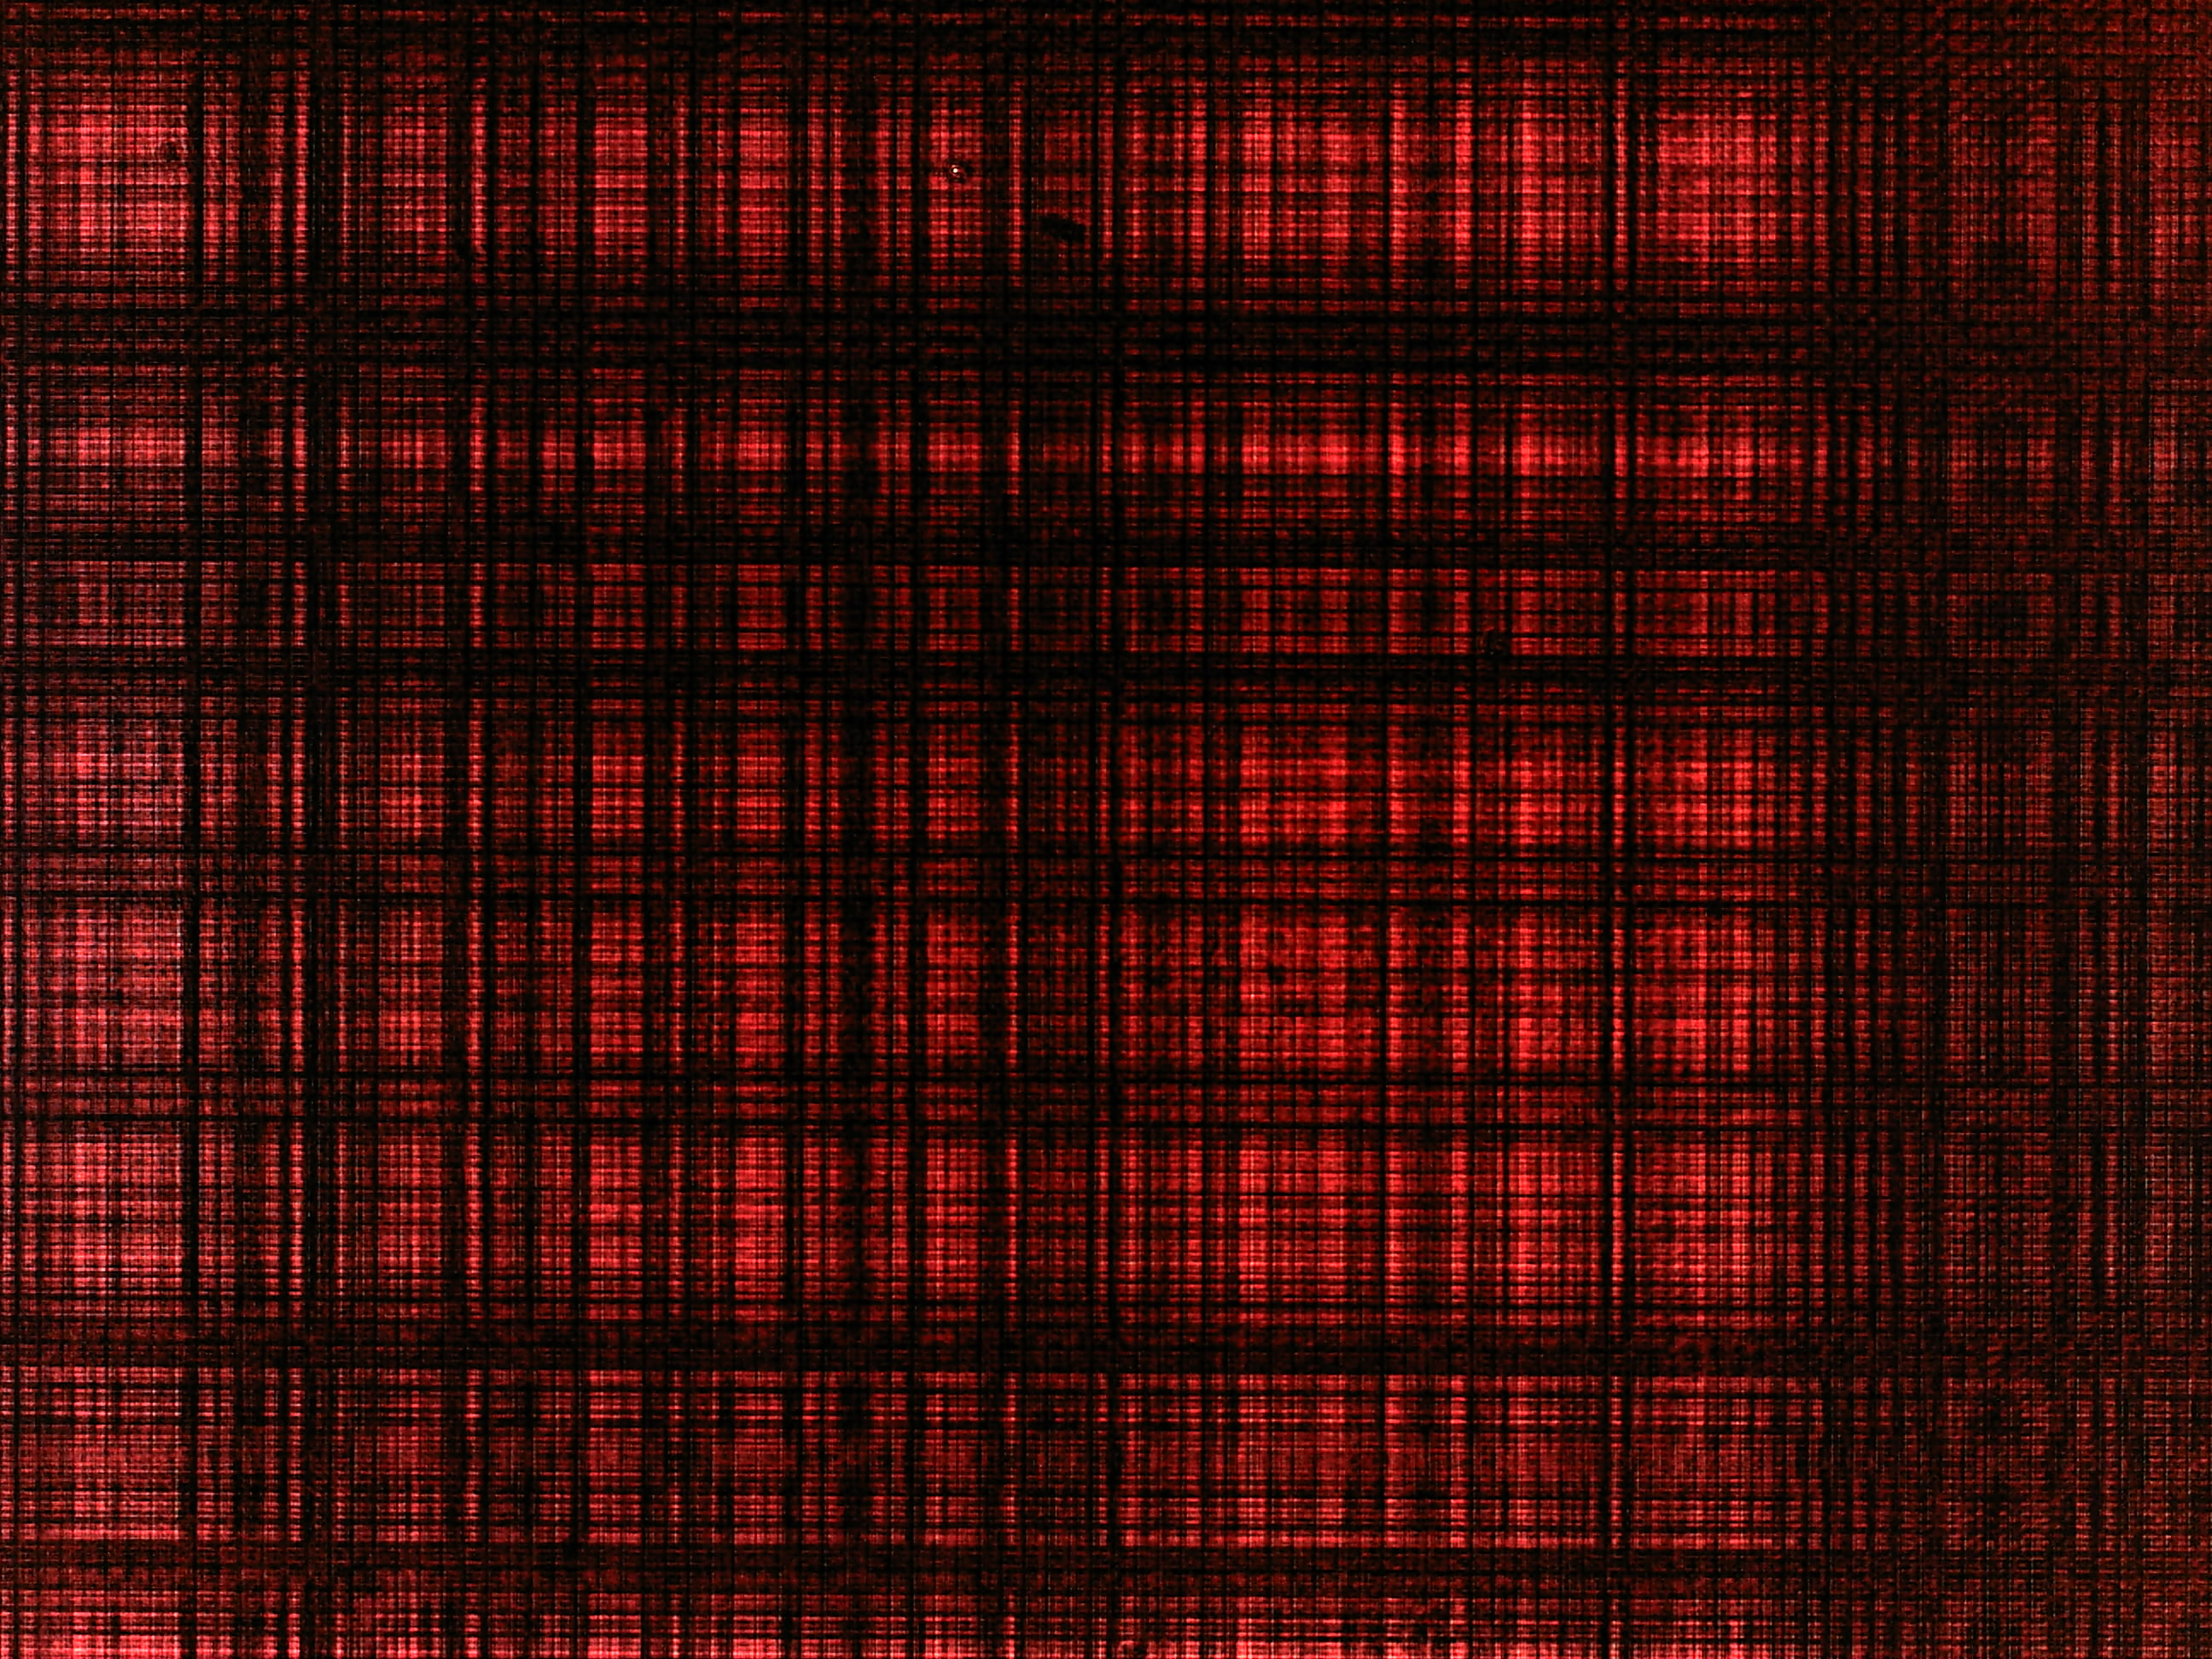
\includegraphics[scale=0.125]{pics/slm/ov5642dtmask.jpg}
\caption{Doubly Toeplitz mask imaged by OV5642}
\label{fig:dt_ov5642}
\end{figure}
It can be seen in figure \ref{fig:dt_ov5642} that OV5642 produces a better image of the mask. In order to compare the performance of OV5642, another web camera(Microsoft LifeCam HD 3000) was disassembled and the mask was imaged(See figure \ref{fig:dt_lifecam}). The difference in redness is due to the saturation level adjustment on LifeCam.
\begin{figure}[h]
\centering
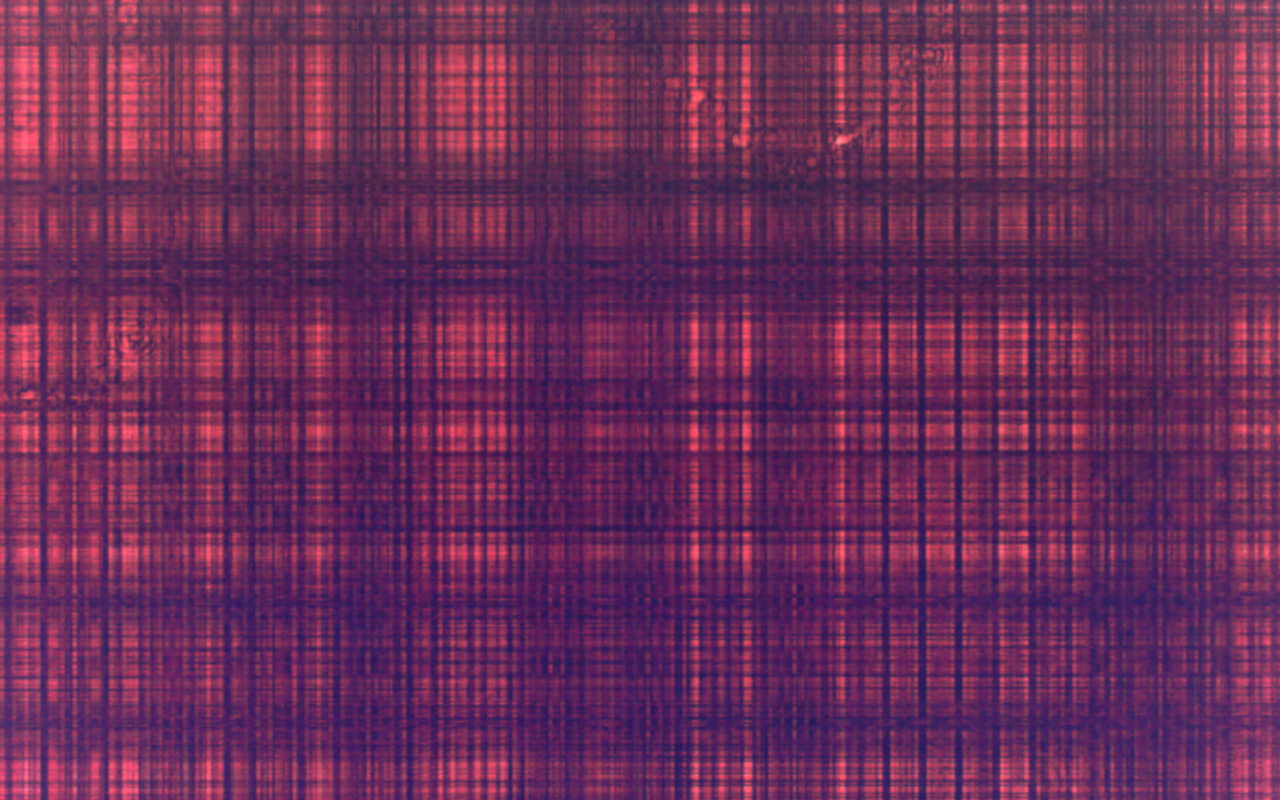
\includegraphics[scale=0.25]{pics/slm/lifecamdtmask.png}
\caption{Doubly Toeplitz mask imaged by Microsoft LifeCam HD 3000}
\label{fig:dt_lifecam}
\end{figure}
A lot of methods were tried to increase the ratio of the first to the second singular value. Firstly, I tried to capture the image without any mask and capture the noise. I subtracted the noise from the mask image. However, this did not lead to any change in the singular component values. I then tried median filtering the output to reduce the Gaussian noise effects and it increased the singular value ratio with all the CMOS sensors. This is shown in table \ref{tbl:dt_cmos_sensor_perf}. Table \ref{tbl:dt_cmos_sensor_perf} was plotted from the average of images in a particular data set using the same masks. The red channel data and the grayscale image data from the mask image are used for SVD. It can be been from the table that OV2640 provides a better singular value ratio than OV5642. However, the highest singular component does not at all represent the mask that is programmed into the SLM. So, OV2640 does not perform equivalent to OV5642 despite the higher ratio of a singular component.
\begin{center}
\begin{table}[h]
\centering
\begin{tabular}{|l|*{4}{c|}}\hline
\backslashbox{Sensor}{Technique}&\makebox[4em]{SVD(Red)}&\makebox[6em]{\makecell{SVD(Red) \\with \\filtering}}&\makebox[4em]{SVD(Gray)}&\makebox[6em]{\makecell{SVD(Gray) \\with \\filtering}}\\\hline
\makebox[3em]{OV2640}&\makebox[3em]{7.833}&\makebox[3em]{11.16}&\makebox[3em]{8.05}&\makebox[3em]{10.49}\\\hline
\makebox[3em]{OV5642}&\makebox[3em]{8.74}&\makebox[3em]{10.84}&\makebox[3em]{7.04}&\makebox[3em]{10.78}\\\hline
\makebox[3em]{LifeCam}&\makebox[3em]{16.82}&\makebox[3em]{21.57}&\makebox[3em]{20.89}&\makebox[3em]{26.75}\\\hline
\end{tabular}
\caption{Performance of Different CMOS sensors(The values indicate the ratio of the first SVD to the second SVD value)}
\label{tbl:dt_cmos_sensor_perf}
\end{table}
\end{center}
The same results as in the simulation(only one singular value) could not be replicated because the mask that is produced by the SLM is not completely binary as observed in the previous experiment with SLM. If you observe the images from the sensor closely you can see that the black regions allow some portion of the light to pass through. This results in the image matrix becoming non-binary which in-turn results in secondary SVD components. One way to solve this would be to use a threshold and make the mask image binary but this would result in loss of diffraction and object data. Apart from this factor, another reason why other SVD components are observed is due to the presence of dead-pixel regions in the output data. The values of these pixels over-ride the values of the mask. These effects do not play a major role in lens-based imaging but form a very important role in lensless imaging. Exposure plays a very important role in the decomposability of the matrix. I first thought of increasing the exposure in order to make the difference between the black and white more prominent (which in-turn increases separability). This idea seems to have worked out. The ratio of singular value to the exposure time is shown in Figure \ref{fig:svd_exposure}. The mask becomes separable as the exposure time is increased. However, this comes at a disadvantage. LifeCam has a very limited controllable range of exposure time and the sensor starts quickly saturating at around 2 $ms$. When the sensor starts saturating, it leads to loss of data which in turn will have an effect on reconstruction. The next step would be to estimate the system matrices $M_x$ and $M_y$ which is described in the next chapter. 
\begin{figure}[h]
\centering
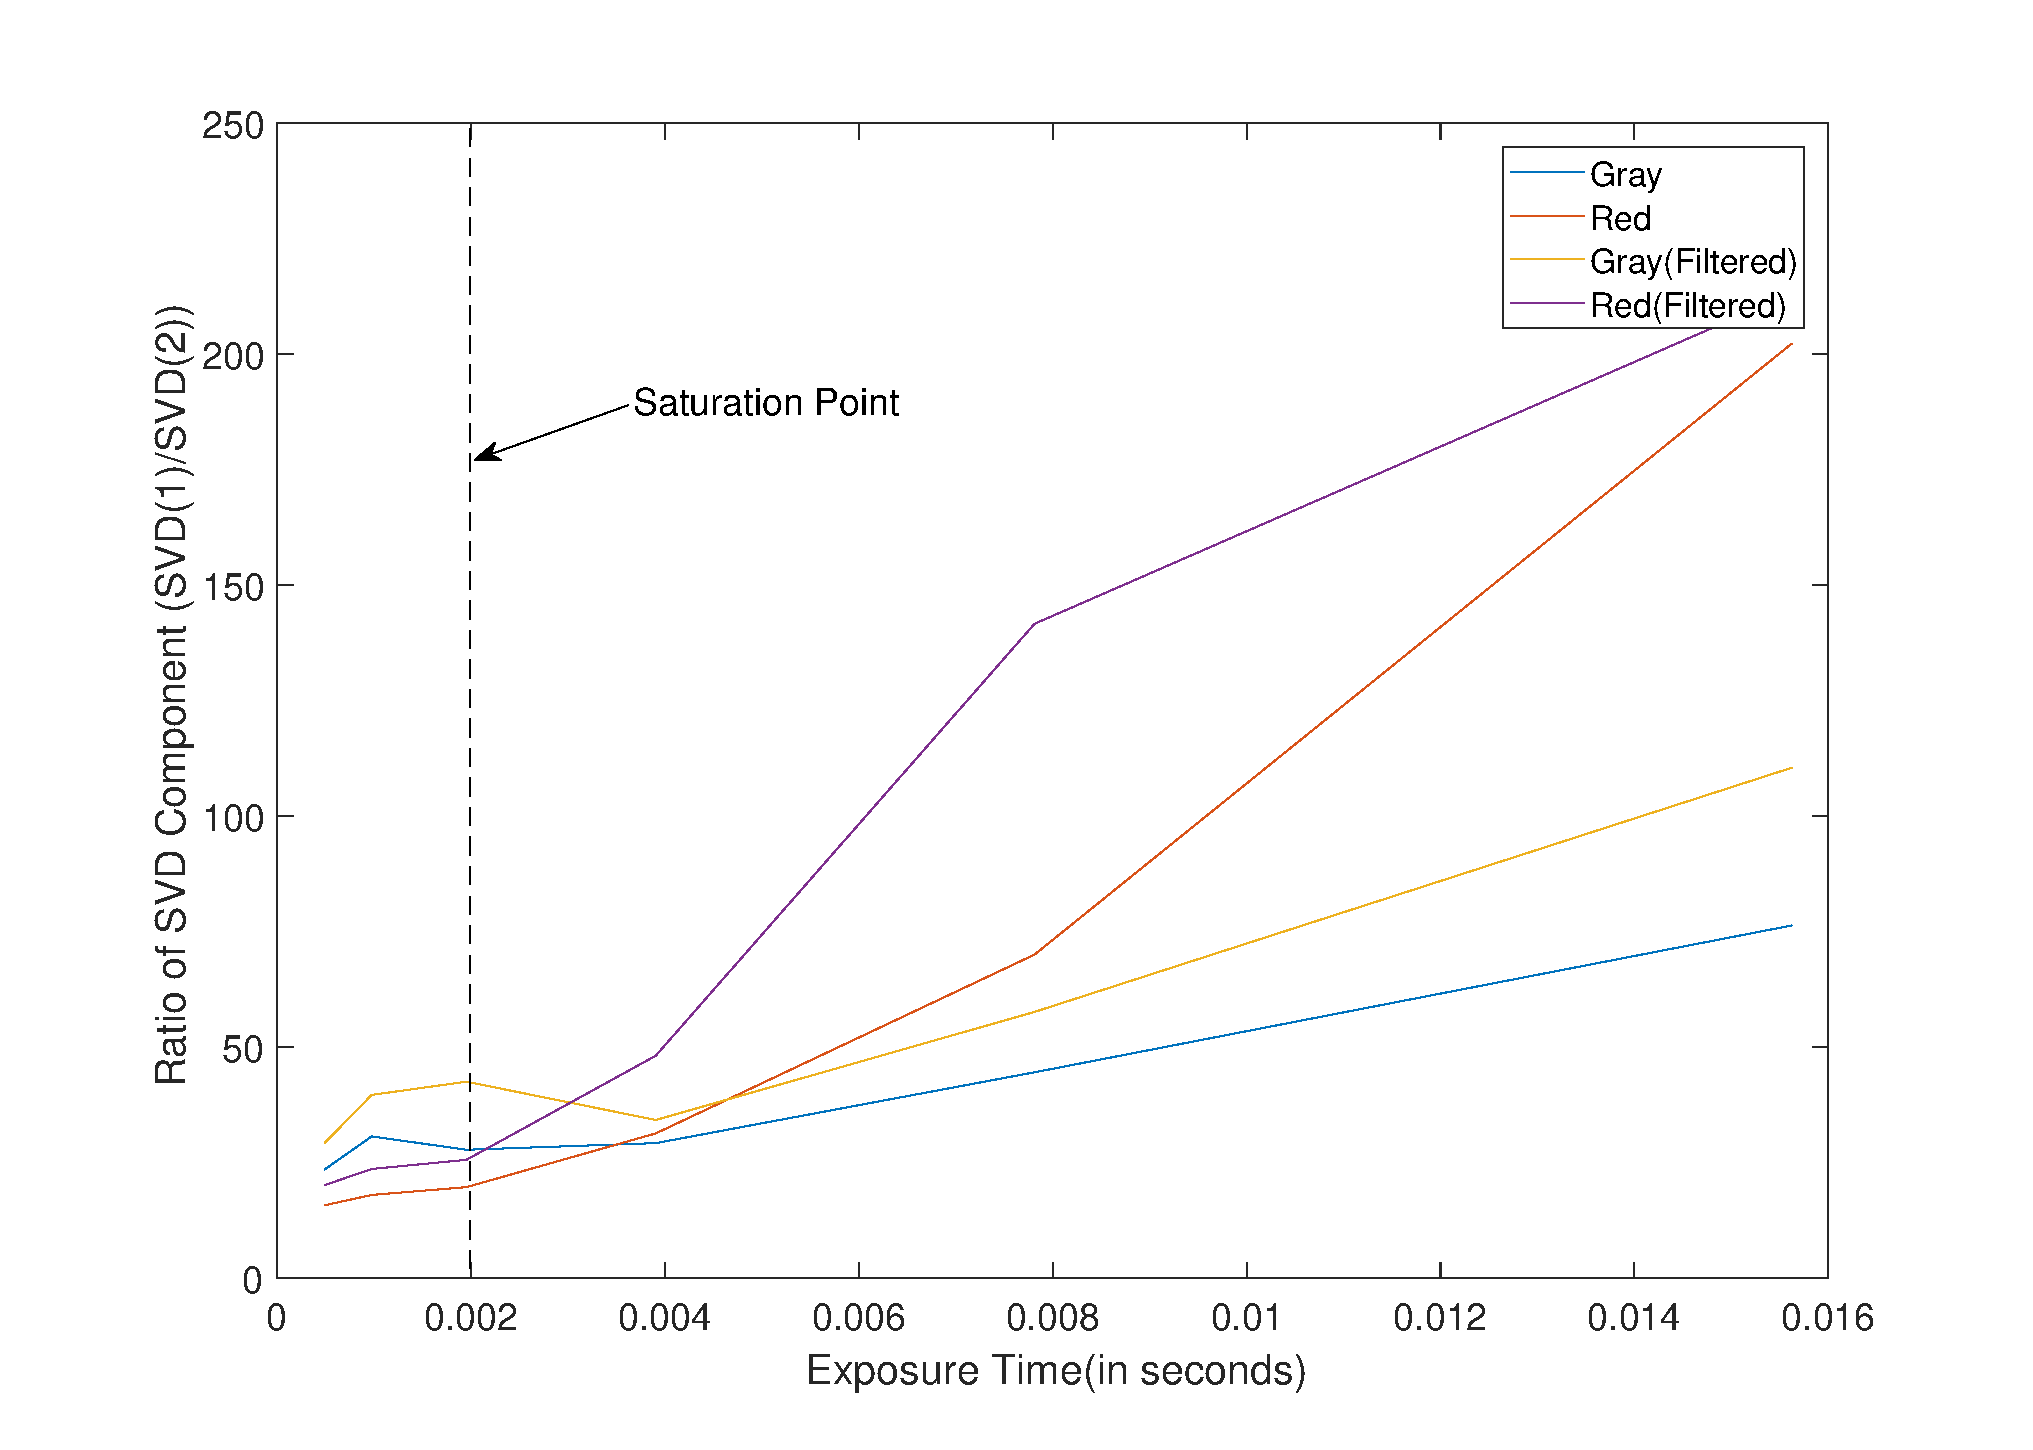
\includegraphics[width = \linewidth]{pics/slm/svd_graph_exposure}
\caption{Impact of Exposure Time on Singular Values}
\label{fig:svd_exposure}
\end{figure}
The best decomposition that I could get was using the LifeCam HD-3000 with exposure adjusted(without saturation) based on figure \ref{fig:svd_exposure}. The decomposition of the mask into different components is shown in figure \ref{fig:svd_dec_exp}. 
\begin{figure}[ht]
\centering
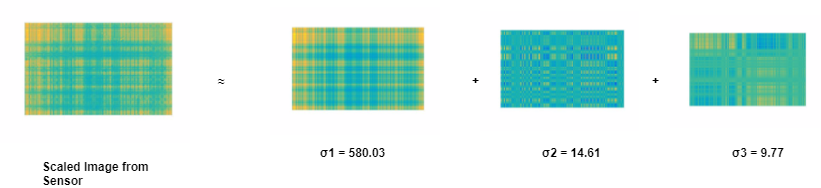
\includegraphics[width = \linewidth, height = 6cm]{pics/slm/svd-decomp-exp.png}
\caption{Decomposition of best data set(Ratio of first to second component = 39.70 )}
\label{fig:svd_dec_exp}
\end{figure}